\documentclass[10pt,aspectratio=1610,compress,dvipsnames]{beamer}
\usepackage{kotex}
\usetheme[
%%% option passed to the outer theme
%    progressstyle=fixedCircCnt,   % fixedCircCnt, movingCircCnt (moving is deault)
]{Feather}

% If you want to change the colors of the various elements in the theme, edit and uncomment the following lines

% Change the bar colors:
%\setbeamercolor{Feather}{fg=red!20,bg=red}

% Change the color of the structural elements:
%\setbeamercolor{structure}{fg=red}

% Change the frame title text color:
%\setbeamercolor{frametitle}{fg=blue}

% Change the normal text color background:
%\setbeamercolor{normal text}{fg=black,bg=gray!10}

%-------------------------------------------------------
% INCLUDE PACKAGES
%-------------------------------------------------------

%\usepackage[utf8]{inputenc}
%\usepackage[spanish,es-tabla]{babel}
%\usepackage[T1]{fontenc}
\usepackage{helvet}

%\usepackage[T1]{fontenc}
%\usepackage[utf8]{inputenc}
%\usepackage{newpxtext}
%\usepackage{newpxmath}

\usepackage[T1]{fontenc}
\usepackage[utf8]{inputenc}
\usepackage{textcomp}
\renewcommand{\ttdefault}{lmtt} % 

%\usepackage{fontspec}
%\setmainfont{TeX Gyre Termes}
%\setsansfont[
%Path = fonts/,
%UprightFont = *Medium.ttf,
%BoldFont    = *Bold.ttf,
%AutoFakeSlant = 0.2
%]{GmarketSansTTF}
%\setmainhangulfont[
%Path = fonts/,
%UprightFont = *Medium.ttf,
%BoldFont    = *Bold.ttf,
%AutoFakeSlant = 0.2
%]{GmarketSansTTF}
%\usepackage{textcomp}
%\renewcommand{\ttdefault}{lmtt} % 

\usepackage{soul}

%-------------------------------------------------------
% DEFFINING AND REDEFINING COMMANDS
%-------------------------------------------------------
% colored hyperlinks
\newcommand{\chref}[2]{
	\href{#1}{{\usebeamercolor[bg]{Feather} #2}}
}

\makeatletter
\def\blfootnote{\gdef\@thefnmark{}\@footnotetext}
\makeatother

%-------------------------------------------------------
% THE BODY OF THE PRESENTATION
%-------------------------------------------------------

\usepackage{listings} % For code highlighting with lstlisting

\usepackage{tikz}
\usepackage{pgfplots, pgfplotstable}
\usetikzlibrary{positioning, shapes.geometric, arrows}
\usetikzlibrary{patterns} % Load the patterns library
\usetikzlibrary{positioning} % Load the positioning library
\usetikzlibrary{decorations.markings, arrows.meta}
\usetikzlibrary{decorations.pathmorphing}
\usetikzlibrary{bending, shadows.blur}
\usetikzlibrary{fit, calc, shapes}
\usetikzlibrary{mindmap}
\usetikzlibrary{tikzmark}

\usepackage{multicol}
\renewcommand{\lstlistingname}{Code}
\usepackage{array}
\usepackage{booktabs}
\usepackage{adjustbox}
\usepackage{kotex}
\usepackage{soul}

\usepackage{amssymb,amsmath}
\usepackage{tabularx}
\usepackage{multirow}
\usepackage{amssymb,amsmath,amsthm,commath, amsfonts}
\usepackage{kotex}

\usepackage{pdfrender}
%-------------------------------------------------------
% INFORMATION IN THE TITLE PAGE
%-------------------------------------------------------

\title[The UNAM Feather Beamer Theme] % [] is optional - is placed on the bottom of the sidebar on every slide
{ % is placed on the title page
	\textbf{\Huge {\color{magenta}} SoK: Computer-Aided Cryptography}\\ [.25cm]
	%{\rmfamily\large by }
%		\textbf{\fontsize{15.8}{16}\selectfont Verifying cryptographic implementations with Jasmin \& EasyCrypt}
}
\subtitle[The Feather Beamer Theme]
{
	\text{\large \textbf{KeyWord:} Computer-aided cryptography, Design-Level Security,}
	\\ \text{\large Symbolic Tool, Computational Tool, Functional Correctness and Efficiency}
}

\definecolor{namegold}{HTML}{fdb515}
\definecolor{namegold2}{HTML}{f78708}
\author[Author Name]
{   
	\vspace{.5cm}
	\textbf{\fontsize{14}{10}\sffamily Ji, Yonghyeon} \\ [.2cm]
	\color{black} 
	\texttt{hacker3740@kookmin.ac.kr}
}
\definecolor{co2blue}{HTML}{9ac2e6}
\definecolor{co2green}{HTML}{e2f0d9}
\definecolor{co2orange}{HTML}{ffbf03}

\institute[UNAM]
{
	\vspace{-.5cm}
	\textbf{\fontsize{13}{14}\sffamily Department of Cyber Security}\\
	\fontsize{13}{14}\sffamily Kookmin University\\
	\vspace{0.2cm}
	
\includegraphics[scale=0.2]{Feathergraphics/Ciencias-Quimicas.png} \\
	\vfill
	\vspace{-1cm}
}

\date{April 29, 2026}
\input{tcolorbox}
\input{listing}
% Pseudo-code
\usepackage[linesnumbered,ruled]{algorithm2e}
\usepackage{algorithmicx}
\usepackage{algpseudocode}
%\usepackage{setspace}
\SetKwComment{Comment}{/* }{ */}
\SetKwProg{Fn}{Function}{:}{end}
\SetKwProg{Procedure}{Procedure}{:}{end}
\SetKwProg{Alg}{Algorithm}{:}{end}
\SetKw{End}{end}
\SetKw{DownTo}{downto}

% Define a new environment for algorithms without line numbers
\newenvironment{algorithm2}[1][]{
	% Save the current state of the algorithm counter
	\newcounter{tempCounter}
	\setcounter{tempCounter}{\value{algocf}}
	% redefine the algorithm numbering (remove prefix)
	\renewcommand{\thealgocf}{}
	\begin{algorithm}
	}{
	\end{algorithm}
	% Restore the algorithm counter state
	\setcounter{algocf}{\value{tempCounter}}
}
\newcommand{\F}{\mathbb{F}}
\newcommand{\Z}{\mathbb{Z}}

\newcommand{\gen}[1]{\langle #1\rangle}

\newcommand{\algo}{\mathcal{A}}
\newcommand{\Adv}{\mathrm{Adv}}
\newcommand{\Func}{\mathrm{Func}}
\newcommand{\Prob}{\Pr}
\newcommand{\bits}{\{0,1\}}
\newcommand{\negl}{\mathrm{negl}}
\newcommand{\KeyGen}{\mathsf{KeyGen}}
\newcommand{\Enc}{\mathsf{Enc}}
\newcommand{\Dec}{\mathsf{Dec}}
\newcommand{\Sign}{\mathsf{Sign}}
\newcommand{\Ver}{\mathsf{Ver}}
\newcommand{\Tag}{\mathsf{Tag}}
\newcommand{\Gen}{\mathsf{Gen}}
%\newcommand{\VerOracle}{\mathsf{VerOracle}}
%\newcommand{\GenOracle}{\mathsf{GenOracle}}
\newcommand{\VerOracle}{\mathcal{O}^{\mathsf{MAC}\text{-}\mathsf{Ver}}}
\newcommand{\GenOracle}{\mathcal{O}^{\mathsf{MAC}\text{-}\mathsf{Gen}}}
\newcommand{\MAC}{\mathsf{MAC}}
\newcommand{\CMAC}{\mathrm{CMAC}}
\newcommand{\dbl}{\mathsf{dbl}}
\newcommand{\MSB}{\mathsf{MSB}}
\newcommand{\xor}{\oplus}
\newcommand{\GF}{\mathsf{GF}}

\usepackage[linguistics]{forest}
\usepackage{stmaryrd}
\usepackage{pifont}

% Scale navigation down only when it overflows; dots remain full-size otherwise.
\newsavebox{\csenavbox}
\setbeamertemplate{headline}{%
  \leavevmode%
  \hbox{%
    \begin{beamercolorbox}[wd=\paperwidth,ht=2.5ex,dp=3.125ex]{palette quaternary}%
      \savebox{\csenavbox}{\insertnavigation{\paperwidth}}%
      \ifdim\wd\csenavbox>\paperwidth
        \resizebox{\paperwidth}{!}{\usebox{\csenavbox}}%
      \else
        \usebox{\csenavbox}%
      \fi
    \end{beamercolorbox}%
  }%
  \featherheaderbackground
}

\begin{document}

%-------------------------------------------------------
% THE TITLEPAGE
%-------------------------------------------------------

{\1% % this is the name of the PDF file for the background
\begin{frame}[plain,noframenumbering] % the plain option removes the header from the title page, noframenumbering removes the numbering of this frame only
  \titlepage % call the title page information from above
\end{frame}}

%-------------------------------------------------------
\begin{frame}{\textbf{Contents}}
\tableofcontents
\end{frame}
%-------------------------------------------------------
\section{I. Introduction}
\begin{frame}[plain]% The optional argument 'plain' hides the headline and footline
\begin{center}\bfseries\centering
	
\includegraphics[scale=1]{Feathergraphics/cse_logo_opa10}
	\vspace{-5.75cm} \\
	{\adjustbox{scale=3}{\color{cseblue} I. Introduction}}
	\bigskip\bigskip % Vertical whitespace
	{\ }\vspace{4cm}\\
	\bigskip
\end{center}
\end{frame}

\begin{frame}[fragile]{\bfseries I. Introduction}{}
\begin{center}
	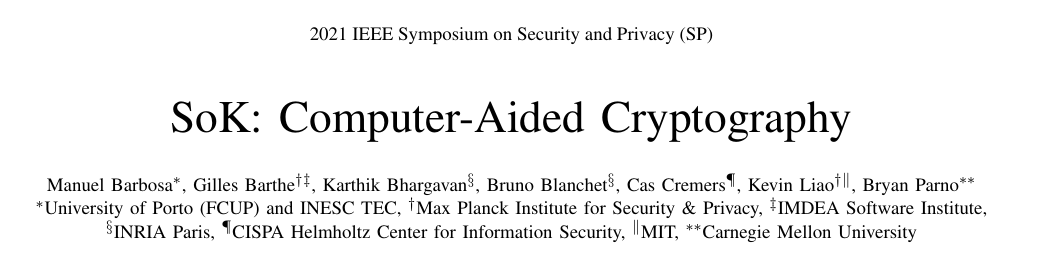
\includegraphics[width=1\textwidth]{images/260422-1}
\end{center}	
%\begin{enumerate}[$\bullet$]
%	\item The paper surveys computer-aided cryptography (CAC): \begin{itemize}
%		\item formal, machine-checkable methods
%		\item for designing, analyzing, implementing, and validating cryptographic mechanisms.
%	\end{itemize} 
%\end{enumerate}
\end{frame}

\begin{frame}[fragile]{\bfseries I. Introduction}{Problem, Prior, and Approach/Direction}
\begin{enumerate}[$\bullet$]
	\item {\bfseries\color{cseblue}Problem:}
	\item[] \textbf{Cryptographic mechanisms} are {\color{red} hard to design, implement, and deploy \underline{correctly (securely)}}, and often fail through flawed proofs, bugs, or side-channel leakage.
\end{enumerate}
\begin{center}
	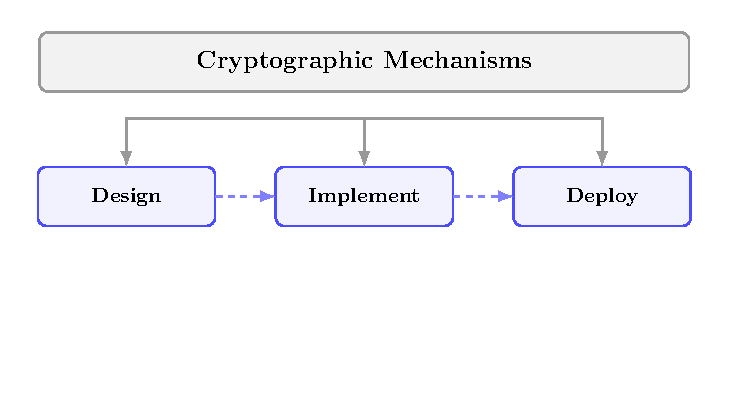
\includegraphics[scale=.9]{illustration/illustration-1.pdf}
\end{center}
\end{frame}

\begin{frame}[fragile]{\bfseries I. Introduction}{Problem, Prior, and Approach/Direction}
\begin{enumerate}[$\bullet$]
	\item {\bfseries\color{cseblue}Problem:}
	\item[] \textbf{Cryptographic mechanisms} are {\color{red} hard to design, implement, and deploy \underline{correctly (securely)}}, and often fail through flawed proofs, bugs, or side-channel leakage.
%	\item[] 
%	\item[]
%	\item {\bfseries\color{cseblue}Prior:}
%	\begin{itemize}
%		\item[]
%		\item Game-based structuring helps, but human checks remain fallible.
%	\end{itemize}
%	\item[] 
%	\item[] 
%	\item {\bfseries\color{cseblue}Approach/Direction:}
%	\begin{itemize}
%		\item[]
%		\item Use formal verification (computer-aided cryptography).
%\end{itemize}
\end{enumerate}
\begin{center}
	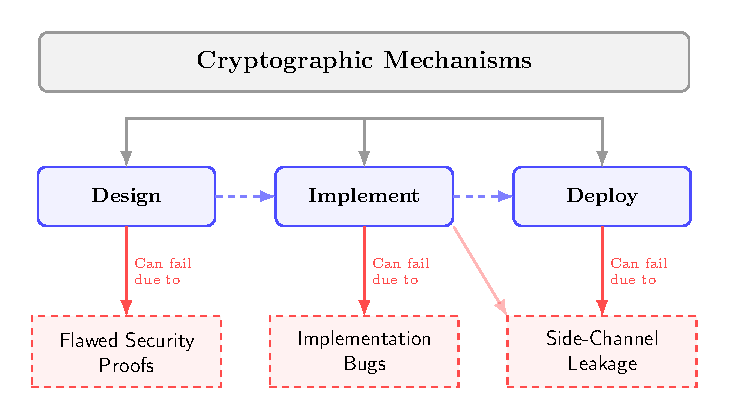
\includegraphics[scale=.9]{illustration/illustration-2.pdf}
\end{center}
\end{frame}

\begin{frame}[fragile]{\bfseries I. Introduction}{Approach}
\begin{enumerate}[$\bullet$]
	\item {\bfseries\color{cseblue}Approach:}
	\item[] The paper systematizes \textbf{computer-aided
	cryptography (CAC)} across three layers:
%	\textbf{design-level security}, \textbf{functional correctness and
%	efficiency}, and \textbf{implementation-level side-channel security}.
\end{enumerate}
\begin{center}
	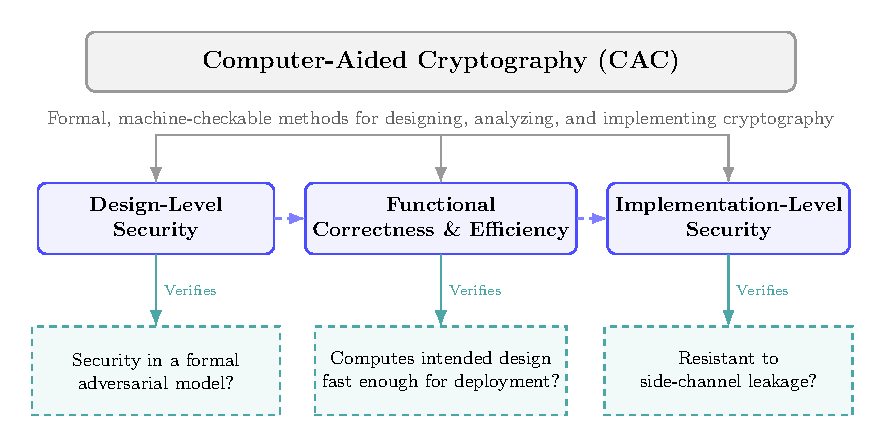
\includegraphics[scale=.9]{illustration/illustration-3.pdf}
\end{center}
\end{frame}

\begin{frame}[fragile]{\bfseries I. Introduction}{Structure of the Paper}
\begin{center}
	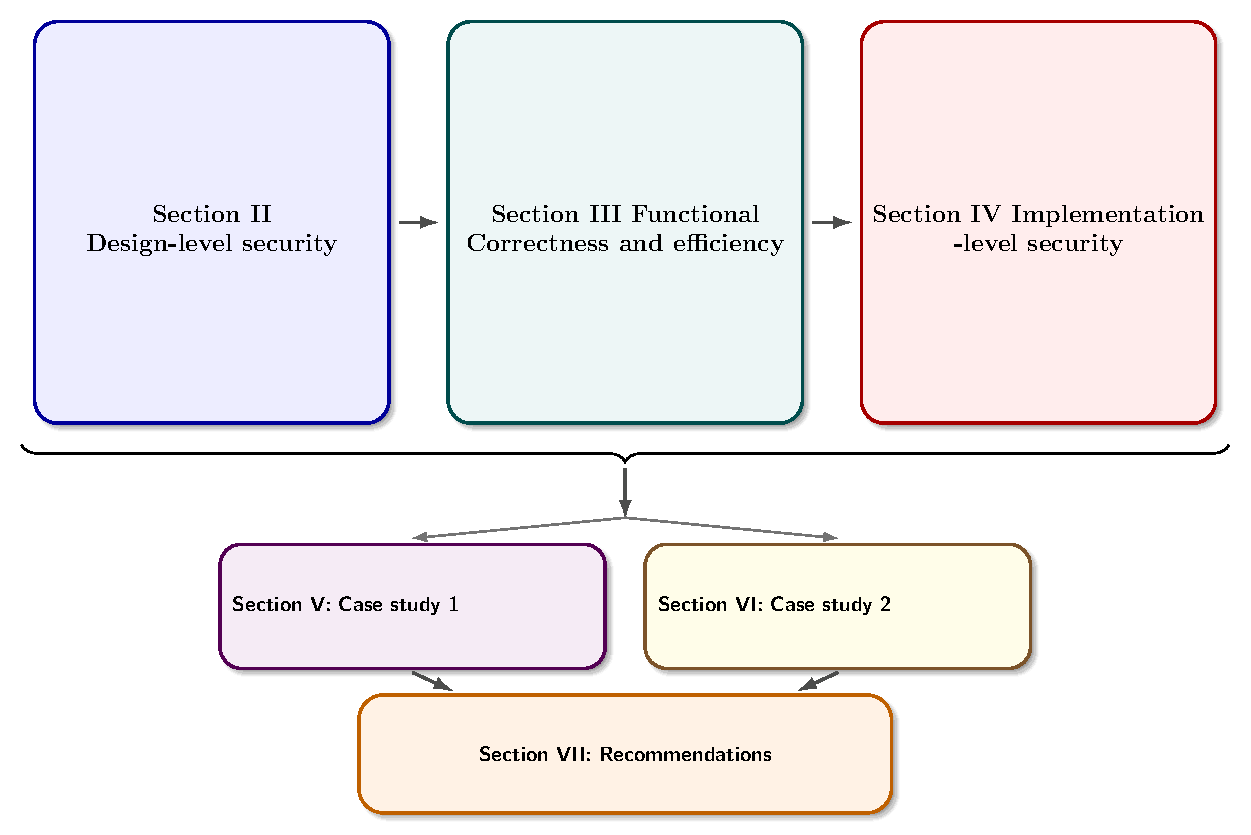
\includegraphics[width=.7\textwidth]{illustration/cac-1.pdf}
\end{center}
\end{frame}

\begin{frame}[fragile]{\bfseries I. Introduction}{How to evaluate several tools?}
%	\begin{description}[style=nextline]
%	\item[Accuracy (A)] How precise is the reasoning? \begin{itemize}
%		\item bounded vs. unbounded session analysis, 
%		\item source vs. assembly level, 
%		\item concrete bounds vs. asymptotic reasoning.
%	\end{itemize}
%	\item[Scope (S)] What properties and systems can be handled? Examples: trace security, equivalence, global state, memory safety, public inputs/outputs, leakage models.
%	\item[Trust (T)] What lies in the trusted computing base? Is the result independently checkable in a theorem prover, or must the tool implementation itself be trusted?
%	\item[Usability (U)] What is the automation level? How natural is the specification language? Is synthesis or interactive proof support available?
%\end{description}
\begin{description}[style=nextline]
	\item[\textbf{Accuracy (A)}] How strong/accurate the guarantee is?
	\item[]
	\item[\textbf{Scope (S)}] What the tool can express and analyze?
	\item[]
	\item[\textbf{Trust (T)}] How much confidence we have in the result?
	\item[]
	\item[\textbf{Usability (U)}] How practical the tool is for users ?
\end{description}
\end{frame}

% =============================================================================
% =============================================================================
% =============================================================================
\section{II. Design-Level Security; Symbolic Tools}
\begin{frame}[plain]% The optional argument 'plain' hides the headline and footline
	\begin{center}\bfseries\centering
		
\includegraphics[scale=1]{Feathergraphics/cse_logo_opa10}
		\vspace{-5.75cm} \\
		{\adjustbox{scale=3}{\color{cseblue} II. Design-Level Security}}
		\bigskip\bigskip % Vertical whitespace
		{\ }\vspace{4cm}\\
		\bigskip
	\end{center}
\end{frame}

\begin{frame}[fragile]{\bfseries II. Design-Level Security}{The Two Design-Level Paradigms}
\textbf{Design-level security} have been developed in two largely separate communities:
\begin{enumerate}[$\bullet$]
	\item[]
	\item {\color{cseblue}\bfseries Symbolic security} (in the formal methods community)
	\item[]
	\item {\color{cseblue}\bfseries Computational security} (in the cryptography community).
\end{enumerate}
\vfill
%\begin{tikzpicture}
%\node[shape=rectangle, draw=black, fill=cseblue, font=\color{white}, rounded corners=4pt, align=left] {Key Question};
%\end{tikzpicture}
%Given a cryptographic design $\mathcal D$, a security property $\Phi$, an adversary class $\mathcal A$, and a semantic model $\mathcal M$, how can one obtain a reliable theorem establishing the security of $\mathcal D$? \[
%\mathcal D \models_{\mathcal M}^{\mathcal A} \Phi \ ?
%\]
\end{frame}

\begin{frame}[fragile]{\bfseries II. Design-Level Security}{The Two Design-Level Paradigms}
\begin{table}\centering\renewcommand{\arraystretch}{1.25}
\begin{tabular}{l|l|l}
\toprule[1.2pt]
\textbf{Aspect} & \textbf{Symbolic Security} & \textbf{Computational Security} \\ \midrule
Main community  & Formal methods & Cryptography \\ \hline
Main object & Protocol logic & Cryptographic security theorem \\ \hline
Messages & Abstract terms & Bitstrings\\ \hline
\colorbox{magenta!50}{Cryptographic primitives} & Idealized symbolic functions                 & Probabilistic algorithms\\  \hline
\multirow{2}{*}{\colorbox{magenta!50}{Adversary}}   & Symbolic Dolev--Yao style          & Probabilistic polynomial-time\\ 
& adversary & adversary\\ \hline
\multirow{2}{*}{Security style} & Logical reachability & Game-based or\\
&or indistinguishability & simulation-based proof\\ \hline
\multirow{2}{*}{Main strength} & Automation and & Cryptographic soundness and\\ 
& attack discovery & quantitative guarantees\\ \hline
Typical tools            & ProVerif, Tamarin        & CryptoVerif, EasyCrypt \\
\bottomrule[1.2pt]
\end{tabular}
\end{table}
%| Aspect                   | Symbolic Security                            | Computational Security                                   |
%| ------------------------ | -------------------------------------------- | -------------------------------------------------------- |
%| Main community           | Formal methods                               | Cryptography                                             |
%| Main object              | Protocol logic                               | Cryptographic security theorem                           |
%| Messages                 | Abstract terms                               | Bitstrings                                               |
%| Cryptographic primitives | Idealized symbolic functions                 | Probabilistic algorithms                                 |
%| Adversary                | Symbolic Dolev--Yao style adversary          | Probabilistic polynomial-time adversary                  |
%| Security style           | Logical reachability or indistinguishability | Game-based or simulation-based proof                     |
%| Main strength            | Automation and attack discovery              | Cryptographic soundness and quantitative guarantees      |
%| Typical tools            | ProVerif, Tamarin, Scyther, Maude-NPA        | CryptoVerif, EasyCrypt, F(^*), CertiCrypt, CryptHOL, FCF |
\end{frame}

\begin{frame}[fragile]{\bfseries II. Design-Level Security - Symbolic Tools}{Symbolic Security}
\textbf{Basic model.}\; In symbolic security, messages are formal terms. For example: \[
m,\quad k,\quad \Enc(m,k),\quad\Dec(c,k).
\] Cryptographic primitives are treated as \colorbox{-blue}{black-box functions}. For symmetric encryption, one may write:
\[
\mathsf{Dec}(\mathsf{Enc}(m,k),k)=m.
\]

\medskip

\noindent
\textbf{Adversary model.}\; A symbolic adversary is usually a Dolev--Yao style attacker. It can \begin{enumerate}[$\bullet$]
	\item intercept messages;
	\item replay messages;
%%	\item compose new symbolic messages;
%%	\item decrypt only when it has the required key;
%%	\item exploit equations in the specified equational theory.
\end{enumerate}
\end{frame}

\begin{frame}[fragile]{\bfseries II. Design-Level Security - Symbolic Tools}{Symbolic Security}
	\textbf{Security properties.}\; Symbolic security commonly proves two kinds of properties.
	
	\begin{enumerate}[(1)]
		\item[]
		\item \colorbox{-blue}{\textbf{Trace properties.}}\; A trace property says: \begin{center}
			``a bad event never occurs in any execution trace.''
		\end{center}
		\item[$\to$] These are natural for secrecy and authentication.
		\item[]
		\item \colorbox{-blue}{\textbf{Equivalence properties.}}\; An equivalence property says: \begin{center}
			``two protocol executions are indistinguishable to the adversary.''
		\end{center}
		\item[$\to$] This is used for privacy-style goals such as anonymity and vote privacy. 
	\end{enumerate}

	\vfill
	
	\noindent\textbf{Strengths of symbolic security.} Symbolic security is powerful when the question is:
	\begin{center}
	``Is there a logical flaw in this protocol design?''
	\end{center}
\end{frame}

\begin{frame}[fragile]{\bfseries II. Design-Level Security - Symbolic Tools}{Timeline of Tools for Symbolic Security Analysis}
\begin{center}
	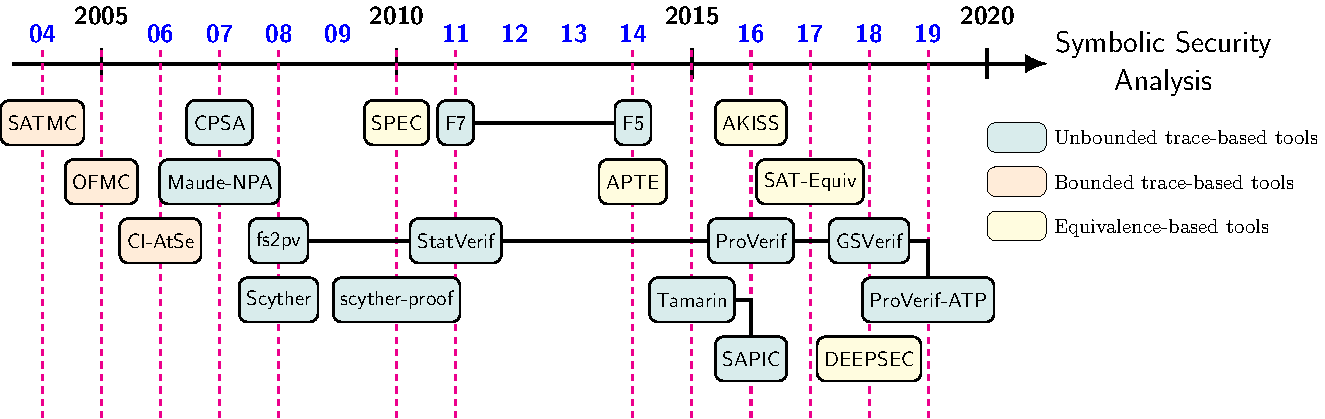
\includegraphics[width=.9\textwidth]{illustration/timeline-symbolic-tools.pdf}
\end{center}

\vfill

\begin{table}[h]
\begin{tabular}{c|c|l}
\toprule
& \textbf{Tool family} & \textbf{Explanation} \\
\midrule
\multirow{2}{*}{One-world} & Unbounded trace & Can we analyze
an unbounded \#(protocol sessions\footnote{sessions = one run of the protocol})? \\
& Bounded trace & Do not consider attacks beyond the cut-off. \\ \midrule
Two-world & Equivalence & Does support verification of equivalence properties? \\
\bottomrule
\end{tabular}
\end{table}
\end{frame}


\begin{frame}[fragile]{\bfseries II. Design-Level Security - Symbolic Tools}{A/S/T/U for Symbolic Tools in Design-Level Security}
\begin{description}[style=nextline]
	\item[\textbf{Accuracy (A)}]\textbf{1. Unbounded Number of Sessions}
	\item[$\to$] A protocol may be secure for ($N$) sessions but insecure for ($N+1$) or more.
	\item[$\to$] An unbounded-session tool gives a stronger, more accurate security claim.
	\item[]
	\item[\textbf{Scope (S)}] \textbf{1. Trace Properties} \\
	\textbf{2. Equivalence Properties}\\ 
	\textbf{3. Equaitional Theories}\\
	\textbf{4. Global Mutable State}
	\item[]
	\item[\textbf{Trust (T)}] \textbf{1. Link to Implementation} \\
	\textbf{2. Independent Verifiability}
	\item[]
	\item[\textbf{Usability (U)}] \textbf{1. Abstractions} \\
	\textbf{2. Interactive Mode} \\ 
	\textbf{3. Specification Language}
\end{description}
\end{frame}

\begin{frame}[fragile]{\bfseries II. Design-Level Security - Symbolic Tools}{A/S/T/U for Symbolic Tools in Design-Level Security}
\begin{description}[style=nextline]
	\item[\textbf{Scope (S)}] \textbf{1. Trace properties} \\
	\item[$\to$] Can it prove that bad events never occur, 
	\item[$\to$] e.g. ``the adversary never learns the session key''?
	\item[]
	\item[] \textbf{2. Equivalence properties}\\
	\item[]
\end{description}
We want to compare two protocols (or two variants of one protocol): \[
P_0\quad\text{vs}\quad P_1.
\] Security means that \begin{center}
	``Adversary $\mathcal A$ cannot distinguish $P_0$ from $P_1$''.
\end{center}
%\begin{enumerate}[$\bullet$]
%	\item Trace properties $\to$ ``nothing bad happens''
%	\item Equivalence properties $\to$ ``two systems look the same to the attacker''
%\end{enumerate}

\end{frame}

\begin{frame}[fragile]{\bfseries II. Design-Level Security - Symbolic Tools}{A/S/T/U for Symbolic Tools in Design-Level Security}
\begin{center}
\begin{minipage}{.525\textwidth}
\begin{description}[style=nextline]
	\item[\textbf{Scope (S)}] \textbf{1. Trace properties}
	\item[] \textbf{2. Equivalence properties}\\
	\item[$\to$] \colorbox{-blue}{Trace equivalence (t)}
	%	\item[] Every trace of one process has an indistinguishable trace of the other.
	\item[$\to$] Open bisimilarity (o)
	%	\item[] Each step of one process can be matched by the other under all attacker inputs.
	\item[$\to$] Diff-equivalence (d)
	%	\item[] Two projections of one biprocess execute in lockstep and differ only by chosen messages.
\end{description}

\medskip

\begin{enumerate}[$\bullet$]
	\item $\mathcal{T}(P)=\mathcal{T}(Q)=\{a,\,ab,\,ac, \varepsilon\}$
	\item $P \approx_{t} Q\iff$ same observable sequences
	\item But structure of branch differs
\end{enumerate}
\end{minipage}\hfill
\begin{minipage}{.47\textwidth}\centering
	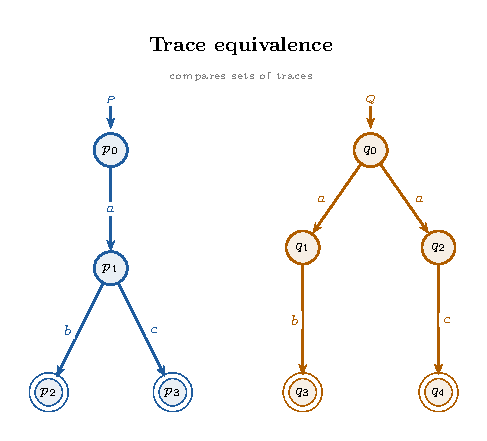
\includegraphics[width=\textwidth]{illustration/symbolic-equ-pro-1.pdf}
\end{minipage}
\end{center}
\begin{center}
\end{center}
\end{frame}

\begin{frame}[fragile]{\bfseries II. Design-Level Security - Symbolic Tools}{A/S/T/U for Symbolic Tools in Design-Level Security}
\begin{center}
\begin{minipage}{.525\textwidth}
\begin{description}[style=nextline]
	\item[\textbf{Scope (S)}] \textbf{1. Trace properties}
	\item[] \textbf{2. Equivalence properties}\\
	\item[$\to$] {Trace equivalence (t)}
	\item[$\to$] \colorbox{-blue}{Open bisimilarity (o)}
	\item[$\to$] Diff-equivalence (d)
\end{description}

\medskip

\begin{enumerate}[$\bullet$]
	\item $P \approx_{o} Q\iff$ step-by-step ind.
\end{enumerate}
\end{minipage}\hfill
\begin{minipage}{.45\textwidth}\centering
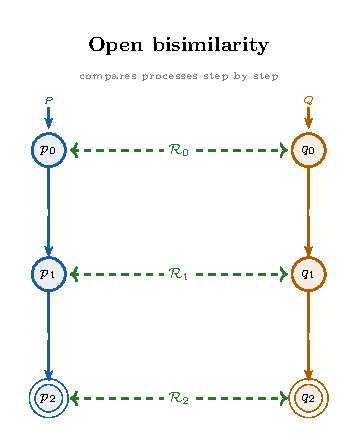
\includegraphics[width=\textwidth]{illustration/symbolic-equ-pro-2.pdf}
\end{minipage}
\end{center}
\begin{center}
\end{center}
\end{frame}

\begin{frame}[fragile]{\bfseries II. Design-Level Security - Symbolic Tools}{A/S/T/U for Symbolic Tools in Design-Level Security}
\begin{center}
\begin{minipage}{.525\textwidth}
\begin{description}[style=nextline]
	\item[\textbf{Scope (S)}] \textbf{1. Trace properties}
	\item[] \textbf{2. Equivalence properties}\\
	\item[$\to$] {Trace equivalence (t)}
	\item[$\to$] {Open bisimilarity (o)}
	\item[$\to$] \colorbox{-blue}{Diff-equivalence (d)}
\end{description}
%\medskip
%\begin{enumerate}[$\bullet$]
%	\item Two protocols have identical structure
%	\item Only differ in data (messages)
%\end{enumerate}

\medskip

\textbf{Example (Real vs Ideal).}\; Consider \[
P_0:\text{send $\mathsf{Enc}(s,k)$}\quad P_1:\text{send $\mathsf{Enc}(r,k)$}
\] where $s$ is the secret and $r$ is a random value. 

If the adversary cannot distinguish $\mathsf{Enc}(s,k)$ and $\mathsf{Enc}(r,k)$, $$P_0\approx_d P_1.$$
\end{minipage}\hfill
\begin{minipage}{.45\textwidth}\centering
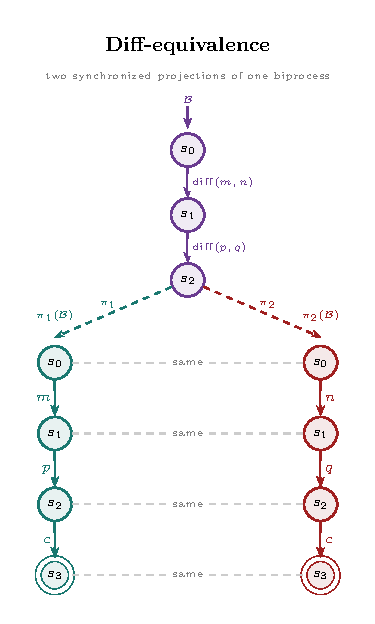
\includegraphics[width=.75\textwidth]{illustration/symbolic-equ-pro-3.pdf}
\end{minipage}
\end{center}
\begin{center}
\end{center}
\end{frame}

\begin{frame}[fragile]{\bfseries II. Design-Level Security - Symbolic Tools}{A/S/T/U for Symbolic Tools in Design-Level Security}
\begin{description}[style=nextline]
	\item[\textbf{Scope (S)}] \textbf{1. Trace properties}
	\item[] \textbf{2. Equivalence properties}
\end{description}
\begin{table}[h]\renewcommand{\arraystretch}{1.5}
\begin{tabular}{l|c|c|c}
	\toprule
	\textbf{Equivalence Properties} & \textbf{Strength} & \textbf{Expressiveness} & \textbf{Automation} \\
	\midrule
	Trace equivalence &	weakest & highest & hardest \\ \hline
	Open bisimilarity &	medium & medium & moderate \\ \hline
	Diff-equivalence & strongest & lowest & easiest \\
	\bottomrule
\end{tabular}
\end{table}
The hierarchy is \begin{center}
diff-equivalence$\implies$open bisimilarity$\implies$trace equivalence.
\end{center} In other words, \[
\approx_d\;\subseteq\; \approx_o\;\subseteq\;\approx_t.
\]
%\begin{enumerate}[$\bullet$]
%	\item diff-equivalence $\to$ fully automatic
%	\item bisimulation $\to$ partially automated
%\end{enumerate}
\end{frame}

\begin{frame}[fragile]{\bfseries II. Design-Level Security - Symbolic Tools}{A/S/T/U for Symbolic Tools in Design-Level Security}
\begin{center}
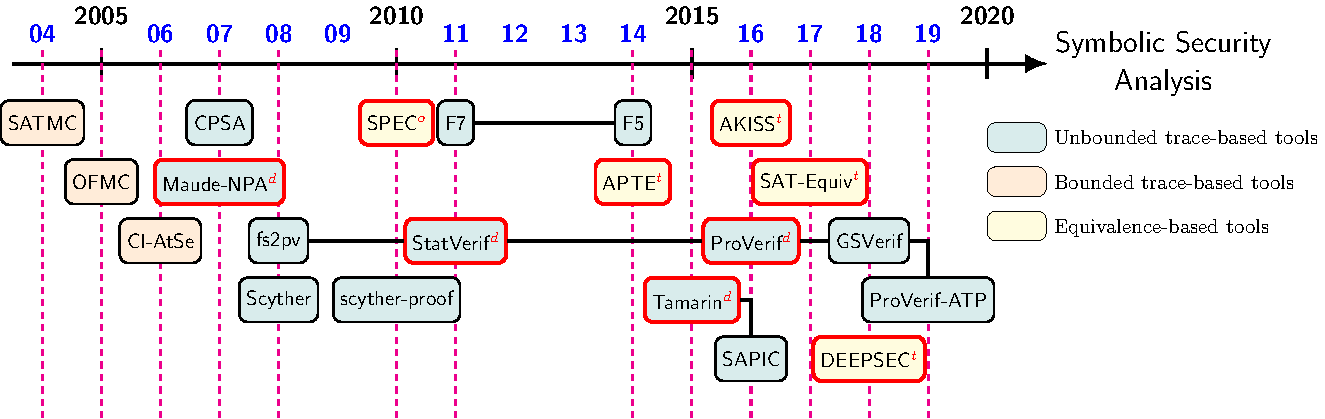
\includegraphics[width=.9\textwidth]{illustration/timeline-symbolic-tools-2.pdf}
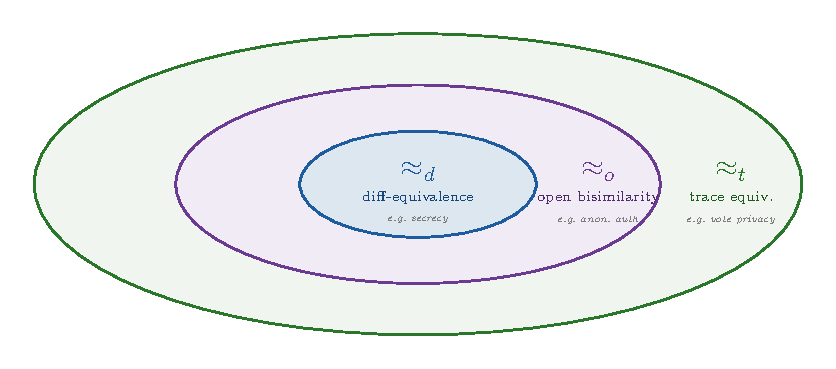
\includegraphics[width=.65\textwidth]{illustration/symbolic-equ-pro-4.pdf}
\end{center}
\end{frame}


\begin{frame}[fragile]{\bfseries II. Design-Level Security - Symbolic Tools}{A/S/T/U for Symbolic Tools in Design-Level Security}
\begin{description}[style=nextline]
	\item[\textbf{Scope (S)}] \textbf{3. Equational theories} \\
	\item[$\to$] How much cryptographic algebra the tool can faithfully model?
	\item[$\to$] It is about the range of mathematical structures the tool can represent.
	\item[]
%	\item[$\to$] For example, symmetric encryption may be modeled by the equation
%	\[
%	\mathsf{dec}(\mathsf{enc}(m,k),k)=m.
%	\] 
%	\item[] \textbf{4. Global mutable state}
%	\item[]
\end{description}
%The paper gives a coarse classification.
\begin{enumerate}
	\item \textbf{Fixed or no equational theories.}\; \[
	\operatorname{dec}(\operatorname{enc}(m,k),k)=m.
	\]
	\item \textbf{User-defined equations without associativity and commutativity.}\;
	\[
	\operatorname{verify}(\operatorname{sign}(m,sk),pk(sk))=m.
	\]
	\item \textbf{User-defined equations with associativity and commutativity.}\; XOR:
	\[
	x\oplus y = y\oplus x,
	\qquad
	(x\oplus y)\oplus z=x\oplus(y\oplus z).
	\]
	For example, from \(m\) and \(m\oplus k\), the adversary derives
	\[
	m\oplus(m\oplus k)
	=
	(m\oplus m)\oplus k
	=
	k.
	\]\\
\end{enumerate}
\end{frame}

\begin{frame}[fragile]{\bfseries II. Design-Level Security - Symbolic Tools}{A/S/T/U for Symbolic Tools in Design-Level Security}
\begin{description}[style=nextline]
	\item[\textbf{Scope (S)}] \textbf{3. Equational theories} \\
	\item[$\to$] AC: Associativity-Commutativity
\end{description}
\begin{center}
	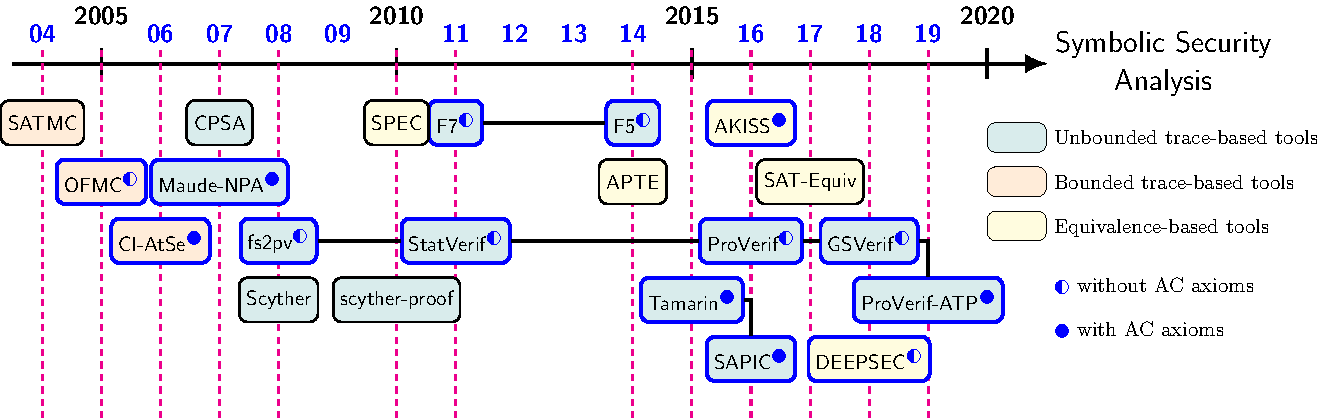
\includegraphics[width=1\textwidth]{illustration/timeline-symbolic-tools-3.pdf}
\end{center}
\begin{description}[style=nextline]
%	\item[]
	\item[] \textbf{4. Global mutable state}
	\item[$\to$] Whether the tool can model \underline{protocols with shared mutable state}, such as databases, key servers, counters, or shared memory.
\end{description}
\end{frame}

\begin{frame}[fragile]{\bfseries II. Design-Level Security - Symbolic Tools}{A/S/T/U for Symbolic Tools in Design-Level Security}
	\begin{description}[style=nextline]
		\item[\textbf{Trust (T)}] \textbf{Link to implementation}\\
		\item[$\to$] Can the tool extract/generate
		\underline{executable code} from specifications in order to \underline{link symbolic}
		security guarantees to implementations?\\
		\item[$\to$] F7, F5, fs2pv \\
		\item[] \; \\
		\textbf{Independent verifiability}
		\item[$\to$] Symbolic tools implement complex algorithms that may contain bugs. 
		\item[$\to$] Independent proof checking reduces the trusted computing base;
		\item[$\to$] scyther-proof\footnote{S. Meier, C. J. F. Cremers, and D. A. Basin, “Strong invariants for
			the efficient construction of machine-checked protocol security proofs,”
			in IEEE Computer Security Foundations Symposium (CSF). IEEE
			Computer Society, 2010, pp. 231–245.}, SPEC\footnote{A. Tiu and J. E. Dawson, “Automating open bisimulation checking for
			the spi calculus,” in IEEE Computer Security Foundations Symposium
			(CSF). IEEE Computer Society, 2010, pp. 307–321.}
		\item[]
%		\item[\textbf{Usability (U)}] \textbf{Abstractions}\\
%		\textbf{Interactive mode} \\
%		\textbf{Independent verifiability} \\
%		\textbf{Specification language}
	\end{description}
\end{frame}

\begin{frame}[fragile]{\bfseries II. Design-Level Security - Symbolic Tools}{A/S/T/U for Symbolic Tools in Design-Level Security}
	\begin{description}[style=nextline]
%		\item[\textbf{Trust (T)}] \textbf{Link to implementation}\\
%		\textbf{Independent verifiability}
%		\item[]
		\item[\textbf{Usability (U)}] \textbf{Abstractions}\\
		\item[$\to$] Does the tool use abstraction? 
		\item[] \;\\
		\textbf{Interactive mode} \\
		\item[$\to$] Does the tool support an interactive analysis mode? 
		\item[] \;\\
		\textbf{Specification language}\\
		\item[$\to$] domain-specific security protocol languages
		\item[$\to$] process calculus
		\item[$\to$] multiset rewriting
		\item[$\to$] general programming language
	\end{description}
\end{frame}

\begin{frame}[fragile]{\bfseries II. Design-Level Security - Symbolic Tools}{OVERVIEW OF TOOLS FOR SYMBOLIC SECURITY ANALYSIS}
\begin{minipage}{.49\textwidth}
	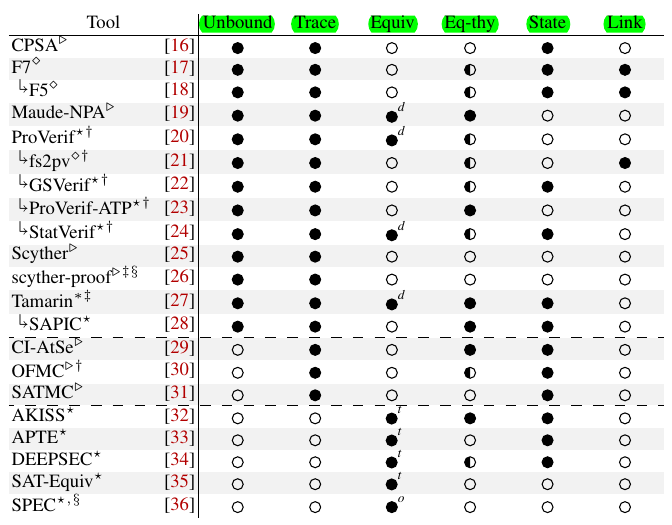
\includegraphics[width=\textwidth]{images/table-1}
\end{minipage}
\begin{minipage}{.49\textwidth}
	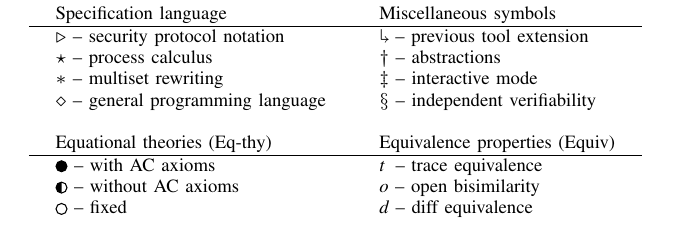
\includegraphics[width=\textwidth]{images/table-1-2}
\end{minipage}
\end{frame}

% -------------------------------------------------------
\begin{frame}[fragile]{\bfseries II. Design-Level Security - Symbolic Tools}{Discussion: Achievements}
\begin{description}[style=nextline]
	\item[{\color{cseblue}\bfseries Achievements}] \textbf{Symbolic proofs for real-world case studies}
\end{description}
\begin{enumerate}[$\bullet$]
	\item \textbf{ProVerif} and \textbf{Tamarin} stand out for scalability and expressivity.
\end{enumerate}
\begin{table}[h]\footnotesize\renewcommand{\arraystretch}{1.3}
\begin{tabular}{l|l|l}
\toprule[1.2pt]
\textbf{Tool} & \textbf{Protocol} & \textbf{Time} \\
\midrule
ProVerif & TLS 1.0 & seconds -- hours \\
ProVerif & TLS 1.3 & $\sim$1 hour \\
ProVerif & Signal & (minutes) -- ($>$1 day) \\
\hline
Tamarin & 5G authentication key exchange & $\sim$5 hours \\
Tamarin & TLS 1.3 & $\sim$1 week, 100\,GB RAM \\
Tamarin & DNP3 SAvS power grid & several minutes \\
Tamarin & Noise protocols & seconds -- hours \\
\bottomrule[1.2pt]
\end{tabular}
\end{table}
\end{frame}

% -------------------------------------------------------
\begin{frame}[fragile]{\bfseries II. Design-Level Security - Symbolic Tools}{Discussion: Challenge}
\begin{description}[style=nextline]
	\item[{\color{cseblue}\bfseries Challenge}] \textbf{Verifying Equivalence Properties}
	\item[$\to$] Equivalence properties are \emph{inherently more difficult} to verify than trace properties --- they involve \textbf{relations between traces}, not single traces.
\end{description}
\medskip
For full automation, one must either:
\begin{enumerate}[(1)]
	\item \textbf{Bound the number of sessions} (loses the unbounded guarantee), or
	\item Use \colorbox{-blue}{\textbf{diff-equivalence}} --- the strongest and most restrictive notion.
\end{enumerate}
\medskip
\begin{enumerate}[$\bullet$]
	\item Diff-equivalence \textbf{cannot} handle many desired properties.
%	, e.g., \textbf{vote privacy} in e-voting and \textbf{unlinkability}.
	\item[]
%	\item {\bfseries\color{cseblue}Recent progress:}
%	\begin{enumerate}[$\to$]
%		\item AKISS, DEEPSEC: support protocols with \texttt{else} branches.
%		\item APTE, AKISS, DEEPSEC: performance via \textbf{partial order reduction}.
%		\item For unbounded sessions + equivalence, diff-equivalence (ProVerif $\to$ Maude-NPA $\to$ Tamarin) remains the \underline{only fully automated approach}.
%	\end{enumerate}
\end{enumerate}
\end{frame}

\section{II. Design-Level Security; Computational Tools}
\begin{frame}[fragile]{\bfseries II. Design-Level Security - Computational Tools}{Timeline of Tools for Computational Security Analysis}
\begin{center}
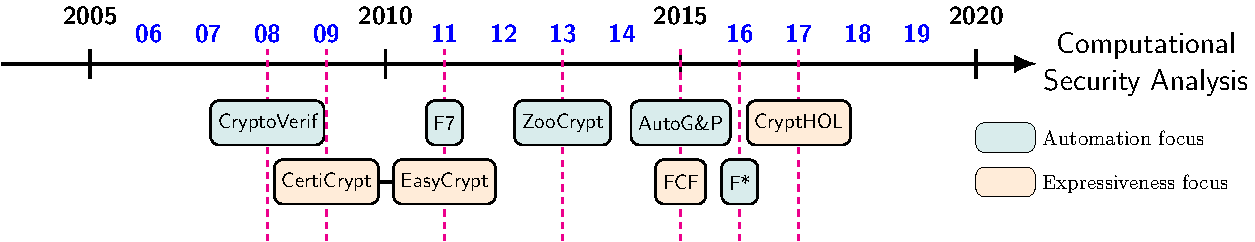
\includegraphics[width=1\textwidth]{illustration/timeline-computational-tools-2.pdf}
\end{center}
\vfill
\begin{center}
	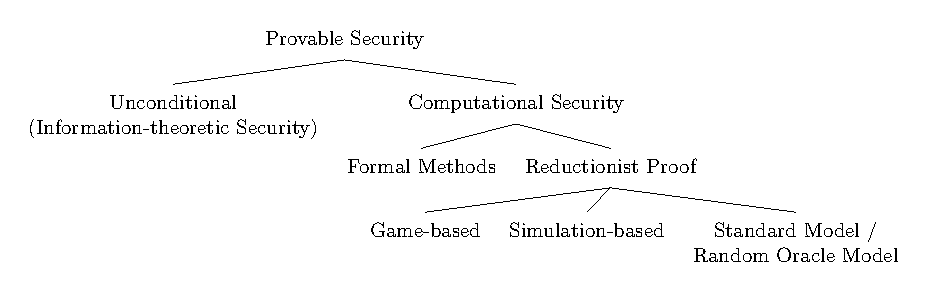
\includegraphics[width=1\textwidth]{illustration/comp-security-1.pdf}
\end{center}
\end{frame}

\begin{frame}[fragile]{\bfseries II. Design-Level Security - Computational Tools}{Design-level Computational Security}
In \textbf{design-level computational security}, \begin{enumerate}[$\bullet$]
	\item the tool is not just searching for symbolic attacks. 
	\item It is helping prove a cryptographic theorem of the following form: \[
	\boxed{\Pr\!\bigl[A\;\text{breaks scheme}\bigr]
	\;\leq\;
	\underbrace{%
		\mathrm{Adv}_{R}(\text{hard primitive})%
	}_{\text{negligible by assumption}}
	\;+\;
	\underbrace{%
		\varepsilon_{\mathrm{stat}}%
	}_{\substack{\text{statistical}\\\text{error}}}}
	\]
\end{enumerate}
%Can every efficient probabilistic adversary be reduced to breaking some assumed-hard primitive?
\end{frame}


\begin{frame}[fragile]{\bfseries II. Design-Level Security - Computational Tools}{A/S/T/U for Computational Tools in Design-Level Security}
\begin{minipage}{.49\textwidth}
\begin{description}[style=nextline]\color{gray!50}
	\item[\color{gray!50}\textbf{Accuracy (A)}]\textbf{1. Unbounded \#(Sessions)}
	\item[]
	\item[\color{gray!50}\textbf{Scope (S)}] \textbf{1. Trace Properties} \\
	\textbf{2. Equivalence Properties}\\ 
	\textbf{3. Equaitional Theories}\\
	\textbf{4. Global Mutable State}
	\item[]
	\item[\color{gray!50}\textbf{Trust (T)}] \textbf{1. Link to Implementation} \\
	\textbf{2. Independent Verifiability}
	\item[]
	\item[\color{gray!50}\textbf{Usability (U)}] \textbf{1. Abstractions} \\
	\textbf{2. Interactive Mode} \\ 
	\textbf{3. Specification Language}\\
	\;
\end{description}
\end{minipage}\hfill\vline\hfill
\begin{minipage}{.49\textwidth}
\begin{description}[style=nextline]
	\item[\textbf{Accuracy (A)}]\textbf{1. Concrete security}
	\item[]
	\item[\textbf{Scope (S)}] \textbf{no separate criterion} \\
	\; \\
	\; \\
	\; \\
	\; \\
	\item[\textbf{Trust (T)}] \textbf{1. Link to Implementation} \\
	\textbf{2. Trusted Computing Base} \\
	\item[]
	\item[\textbf{Usability (U)}] \textbf{1. Reasoning Focus} \\
	\textbf{2. Automated Proof-finding} \\ 
	\textbf{3. Composition}\\ 
	\textbf{4. Specification Language}
\end{description}
\end{minipage}	
\end{frame}

\begin{frame}[fragile]{\bfseries II. Design-Level Security - Computational Tools}{A/S/T/U for Computational Tools in Design-Level Security}
\begin{description}[style=nextline]
	\item[\textbf{Accuracy (A)}]\colorbox{-blue}{\textbf{1. Concrete security}}
\end{description}
\begin{center}
	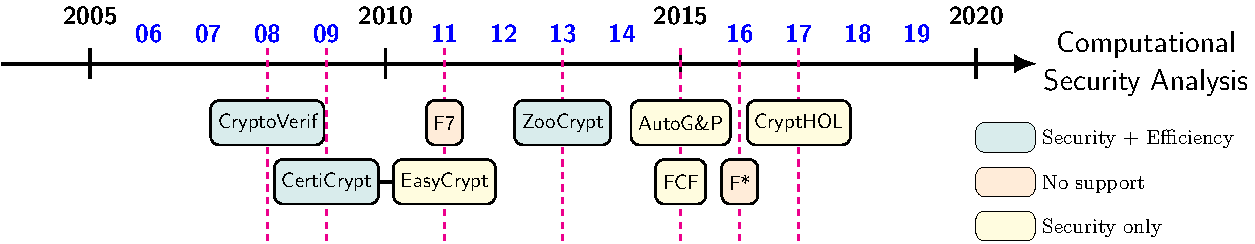
\includegraphics[width=1\textwidth]{illustration/timeline-computational-tools.pdf}
\end{center}
Recall that \[
\boxed{\Pr\!\bigl[A\;\text{breaks scheme}\bigr]
	\;\leq\;
	\underbrace{%
		\mathrm{Adv}_{R}(\text{hard primitive})%
	}_{\text{negligible by assumption}}
	\;+\;
	\underbrace{%
		\varepsilon_{\mathrm{stat}}%
	}_{\substack{\text{statistical}\\\text{error}}}}
\] \textbf{Example.}\; For a MAC with tag length $\tau$, one may want a theorem of the form \[
\mathrm{Adv}_{\Sigma_{\text{PRF}}}^{\text{uf-cma}}(\mathcal{A})\leq {\color{red}\mathrm{Adv}_F^{\text{prf}}(\mathcal{B})}+\frac{q_{\rm ver}}{2^{\tau}}
\] where $q_{\rm ver}$ is the number of forgery attempts.
\end{frame}
\begin{frame}[fragile]{\bfseries II. Design-Level Security - Computational Tools}{A/S/T/U for Computational Tools in Design-Level Security}
\textbf{Theorem (PRF-secure $\implies$ UF-CMA secure).}\; Let $F:\mathcal{K}\times\mathcal{M}\to\set{0,1}^\tau$ be a family of functions. For any UF-CMA adversary $\mathcal{A}$ against $\Sigma_{\text{PRF}}$ asking $q_{\rm ver}$ queries (to $\VerOracle$), there is a PRF adversary against $F$ such that \[
\Adv_{\Sigma_{\text{PRF}}}^{\text{uf-cma}}(\mathcal{A})\leq {\color{red}\Adv_F^{\text{prf}}(\mathcal{B})}+\frac{q_{\rm ver}}{2^{\tau}}.
\]
\textit{Proof.}\; Given $\mathcal{A}$ we build $\mathcal{B}$ as follows:
\begin{center}
	\begin{tabular}{|l|l|}
		\hline
		\textbf{Adversary} $\mathcal{B}$ & \textbf{Subroutine} ${\GenOracle}^\ast(M)$
		\\ \hline
		{\color{gray}1.}\quad $S\gets\varnothing$,\; $(M,T)\gets A^{{\GenOracle}^\ast}$,\; $T'\gets {\rm Fn}(M)$ & 
		{\color{gray}1.}\quad $T\gets\text{Fn}(M)$ \\
		{\color{gray}2.}\quad \textbf{if} $T=T'$ and $M\notin S$ \textbf{then} res $\gets 1$ \textbf{else} res $\gets 0$ &
		{\color{gray}2.}\quad $S\gets S\cup\set{M}$\\
		{\color{gray}3.}\quad \textbf{return} res &
		{\color{gray}3.}\quad \textbf{return} $T$\\
		\hline
	\end{tabular}
\end{center}
Here, ${\rm Fn}\in\set{F_K, \rho}$ where $\rho\gets\Func(\mathcal{M},\set{0,1}^\tau)$. Since \begin{align*}
	\Pr[\text{Ideal$_F$}(\mathcal{B})\Rightarrow 1]
	=\Pr[\rho(M_1)=T_1\lor\cdots\lor \rho(M_{q_{\text{ver}}})=T_{q_{\text{ver}}} ]\leq\sum_{i=1}^{q_{\text{ver}}}\Pr[\rho(M_i)=T_i]= q_{\text{ver}}\cdot 2^{-\tau},
\end{align*} we have \begin{align*}
\Adv_F^{\text{prf}}(\mathcal{B}) &=\Pr[\text{Real$_F$}(\mathcal{B})\Rightarrow 1]-\Pr[\text{Ideal$_F$}(\mathcal{B})\Rightarrow 1]\geq \Adv_{\Sigma}^{\text{uf-cma}}(\mathcal{A})-\frac{q_{\text{ver}}}{2^\tau}.\hfill\qed
\end{align*}
\end{frame}

\begin{frame}[fragile]{\bfseries II. Design-Level Security - Computational Tools}{A/S/T/U for Computational Tools in Design-Level Security}
\begin{description}[style=nextline]	
	\item[\textbf{Accuracy (A)}]\textbf{1. Concrete security}
	\item[]
	\item[\textbf{Scope (S)}] \colorbox{-blue}{\textbf{no separate criterion in the paper}} \\
	\item[]
\end{description}
%The paper’s discussion says 
\begin{enumerate}[$\bullet$]
	\item \;\textbf{[CryptoVerif]} works ell for \underline{protocols such as key exchange}, 
	\item \;\textbf{[EasyCrypt]} closely follows \underline{pen-and-paper game-hopping arguments}.
\end{enumerate}
\begin{description}[style=nextline]	
\item[]
\item[\textbf{Trust (T)}] \colorbox{-blue}{\textbf{1. Link to Implementation}} \\
\item[$\to$] Whether the tool can extract, generate, or verify \underline{executable code} from the specification
%\item[$\to$] so that the computational proof is not merely about a mathematical model.
\item[]
%\textbf{2. Trusted Computing Base} \\
%\item[]
\end{description}
\begin{center}
	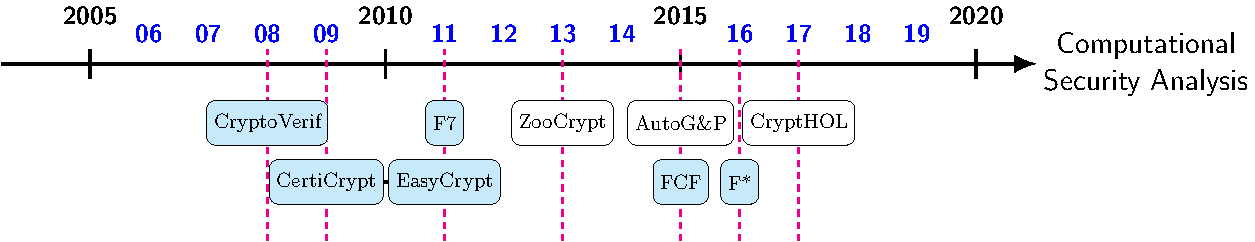
\includegraphics[width=1\textwidth]{illustration/timeline-computational-tools-4.pdf}
\end{center}
\end{frame}


\begin{frame}[fragile]{\bfseries II. Design-Level Security - Computational Tools}{A/S/T/U for Computational Tools in Design-Level Security}
\begin{description}[style=nextline]
%	\item[\textbf{Accuracy (A)}]\textbf{1. Concrete security}
%	\item[]
%	\item[\textbf{Scope (S)}] \textbf{no separate criterion in the paper} \\
%	\item[]
	\item[\textbf{Trust (T)}] {\textbf{1. Link to Implementation}} \\
	\colorbox{-blue}{\textbf{2. Trusted Computing Base}} \\
	\item[]
\end{description}
\begin{center}
	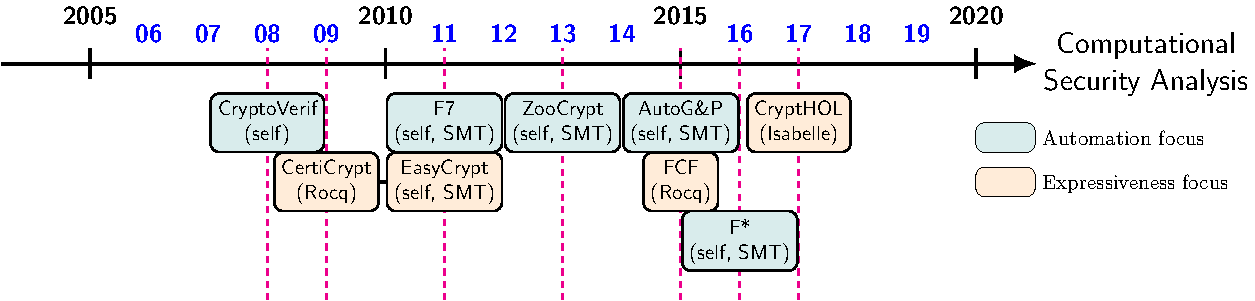
\includegraphics[width=.9\textwidth]{illustration/timeline-computational-tools-3.pdf}
\end{center}
\begin{table}[h]\renewcommand{\arraystretch}{1.25}
\begin{tabular}{l|c|c|c}
	\toprule
	\textbf{} & \textbf{Isabelle} & \textbf{Rocq / Coq} & \textbf{SMT solvers} \\
	\midrule
	Type &	\multicolumn{2}{c|}{Interactive theorem prover} & Automated solver \\ \hline
	Logic & Higher-order Logic (HOL) & CIC\footnote{Calculus of Inductive Constructions} & First-order logic (FOL) \\
	\bottomrule
\end{tabular}
\end{table}
\end{frame}

\begin{frame}[fragile]{\bfseries II. Design-Level Security - Computational Tools}{A/S/T/U for Computational Tools in Design-Level Security}
%\begin{enumerate}[$\bullet$]
%	\item FOL: 
%		``I can talk about objects.''
%	\item HOL:
%		``I can talk about objects, functions, predicates, and sets.''
%	\item CIC :
%		``I can talk about objects, functions, predicates, proofs, programs,
%		and types.''
%\end{enumerate}
\textbf{Example 1 (Associative Law).}\;	Suppose we want to express that a binary operation is associative: 	\[
\boxed{\forall x,y,z.\;(x\cdot y)\cdot z = x\cdot(y\cdot z).}
\]
\begin{enumerate}[$\bullet$]
	\item[FOL] FOL handles this directly. $$\forall x,\forall y,\forall z.\;(x\cdot y)\cdot z = x\cdot(y\cdot z).$$
	\item[]
	\item[HOL] HOL also handles it directly. $$\forall x,y,z:\alpha.\; \mathsf{op}(\mathsf{op}(x,y),z) = \mathsf{op}(x,\mathsf{op}(y,z)).$$ 
%	HOL adds types and lets op be a first-class function.
	\item[]
	\item[CIC] CIC also handles it directly. \[
	A:\mathsf{Type},\qquad \mathsf{op}:A\to A\to A,
	\]
	\[
	\mathsf{assoc}:\forall x,y,z:A,\; \mathsf{op}(\mathsf{op}(x,y),z) = \mathsf{op}(x,\mathsf{op}(y,z)).
	\]
	\item[] 
\end{enumerate}
\end{frame}

\begin{frame}[fragile]{\bfseries II. Design-Level Security - Computational Tools}{A/S/T/U for Computational Tools in Design-Level Security}
\textbf{Example 2 (Natural numbers and Induction).}\; For any subset $A\subseteq\mathbb N$, \[
\begin{cases}
0\in A\\
\forall n\in\mathbb N,\; n\in A\Rightarrow S(n)=n+1\in A
\end{cases}\implies A=\mathbb N.
\]
\begin{enumerate}[$\bullet$]
	\item[FOL] For every first-order formula $\varphi(n)$, \[
	\left[[\varphi(0)] \wedge [\forall n(\varphi(n)\Rightarrow \varphi(Sn))]\right]
	\Rightarrow [\forall n,\varphi(n)].
	\] \textcolor{red}{FOL cannot quantify over arbitrary predicates $\varphi$.}
	\item[]
	\item[HOL] $
	\forall P:\mathbb{N}\to\mathsf{Prop.},\;
	P(0)\Rightarrow (\forall n.\;P(n)\Rightarrow P(Sn)) \Rightarrow \forall n.\;P(n).$
	\item[]
	\item[CIC] $\forall P:\mathsf{nat}\to\mathsf{Type},\;
	P(0)\to (\forall n,\;P(n)\to P(Sn)) \to \forall n,\;P(n).$
	\item[] 
\end{enumerate}
%\begin{lstlisting}[style=shell]
%Inductive nat :=
%	| O : nat
%	| S : nat -> nat.
%\end{lstlisting}
\vfill
\end{frame}

\begin{frame}[fragile]{\bfseries II. Design-Level Security - Computational Tools}{A/S/T/U for Computational Tools in Design-Level Security}
	\begin{description}[style=nextline]
		\item[\textbf{Usability (U)}] \textbf{1. Reasoning Focus} \\
		\item[$\to$] Automation-focused tools;
		\item[$\to$] Expressiveness-focused tools.
		\item[] \;\\
		\textbf{2. Automated Proof-finding} \\ 
		\item[$\to$] Can the tool automatically find security proofs? \\
		\item[$\to$] \textit{AutoG\&P}: proofs of pairing-based schemes.
		\item[$\to$] \textit{CryptoVerif}: proofs of key exchange protocols using a catalog
		of built-in game transformations.
		\item[$\to$] \textit{ZooCrypt}: proofs of padding-based public key encryption schemes.
		\item[] \; \\
		\textbf{3. Composition}\\ 
		\item[$\to$] Does the tool support compositional
		reasoning?\\
		\item[$\to$] \textit{EasyCrypt}, CryptHOL, F7, F$^*$, FCF
%		\textbf{4. Specification Language}
	\end{description}
\end{frame}

\begin{frame}[fragile]{\bfseries II. Design-Level Security - Computational Tools}{A/S/T/U for Computational Tools in Design-Level Security}
	\begin{description}[style=nextline]
		\item[\textbf{Usability (U)}] \textbf{1. Reasoning Focus} \\
		\textbf{2. Automated Proof-finding} \\
		\textbf{3. Composition} \\
		\textbf{4. Specification Language}\\
		\item[$\to$] \textbf{\color{cseblue}Functional.}\; A functional language is natural for defining algorithms: \[
		\mathsf{KeyGen}, \Enc, \Dec\quad \text{or}\quad\mathsf{Hash},\mathsf{Sign},\mathsf{Verify}.
		\] It is good for primitives and functional correctness-style specifications.
		\item[]
		\item[$\to$] \textbf{\color{cseblue}Imperative.}\; An imperative language is natural for game-based proofs like \[
		k\gets\KeyGen();\quad b\xleftarrow{\$}\{0,1\};\quad c\gets\Enc_k(m_b);\quad b'\gets\mathcal A(c);\quad\text{return}\; b=b'.
		\]
	\end{description}
\end{frame}

\begin{frame}[fragile]{\bfseries II. Design-Level Security - Computational Tools}{A/S/T/U for Computational Tools in Design-Level Security}
\begin{table}\centering\renewcommand{\arraystretch}{1.25}
\begin{tabular}{l|l|p{7cm}}
	\toprule[1.2pt]
	\textbf{Category} & \textbf{Criterion} & \textbf{Main question} \\ \midrule
	Accuracy & Concrete security & Does the theorem give explicit \colorbox{-blue}{probability} \colorbox{-blue}{and time bounds}? \\ \hline
	\multirow{2}{*}{Trust} & Link to implementation & Does the proof apply to \colorbox{-blue}{executable code}, or only to an abstract model? \\ \cline{2-3}
	 & Trusted Computing Base & What proof checker, solver, or tool \colorbox{-blue}{implementation must be trusted}? \\ \hline
 	\multirow{4}{*}{Usability} & Reasoning focus & Is the tool focused for \colorbox{-blue}{automation or} \colorbox{-blue}{expressiveness}? \\ \cline{2-3}
	 & Automated proof-finding & Can the tool discover proof? \\ \cline{2-3}
	 & Composition & Can component security theorems be combined \colorbox{-blue}{modularly}? \\ \cline{2-3}
	 & Specification language & Are protocols, games, and algorithms expressed in a natural language?\\
	\bottomrule[1.2pt]
\end{tabular}
\end{table}
\end{frame}

\begin{frame}[fragile]{\bfseries II. Design-Level Security - Computational Tools}{OVERVIEW OF TOOLS FOR COMPUTATIONAL SECURITY ANALYSIS}
\begin{center}
	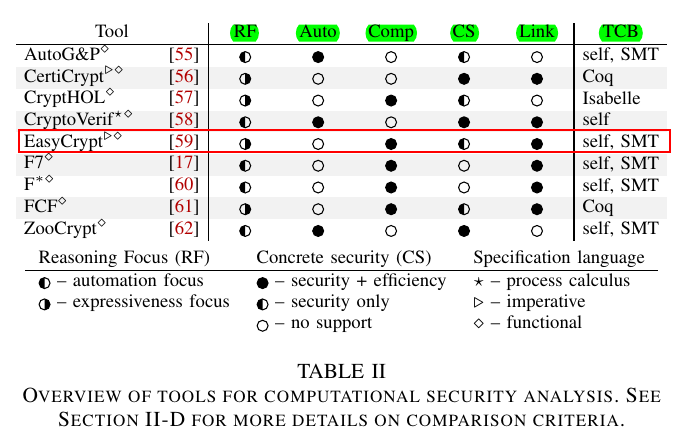
\includegraphics[width=.8\textwidth]{images/table-2}
\end{center}
\end{frame}

% -------------------------------------------------------
\begin{frame}[fragile]{\bfseries II. Design-Level Security - Computational Tools}{Discussion: Achievements}
\begin{description}[style=nextline]
	\item[{\color{cseblue}\bfseries Achievements}] \textbf{Machine-checked security for real-world cryptographic designs}
\end{description}
\begin{table}[h]\footnotesize\renewcommand{\arraystretch}{1.3}
\begin{tabular}{l|l|l}
\toprule[1.2pt]
\textbf{Tool} & \textbf{Protocol / System} & \textbf{Property verified} \\
\midrule
CryptoVerif & TLS 1.3, Signal, WireGuard & Computational security \\
EasyCrypt   & Amazon AWS key management & Computational security \\
EasyCrypt   & SHA-3 standard & Functional + security \\
F7          & miTLS (TLS 1.2) & Computational security at code level \\
F*          & TLS 1.3 record layer & Security + implementation \\
\bottomrule[1.2pt]
\end{tabular}
\end{table}
\end{frame}

% -------------------------------------------------------
\begin{frame}[fragile]{\bfseries II. Design-Level Security - Computational Tools}{Discussion: Takeaways per Tool}
\begin{description}[style=nextline]
%	\item[{\color{cseblue}\bfseries CryptoVerif}] \textbf{Good for highly automated computational analysis of protocols.}
%	\item[$\to$] Both proof-\emph{finding} and proof-\emph{checking}. Based on applied $\pi$-calculus --- natural for protocols exchanging messages in sequence.
%	\item[$\to$] Carefully crafted security assumptions enable \emph{automated discovery} of proof steps.
%	\item[]
%	\item[{\color{cseblue}\bfseries F*}] \textbf{Good for full protocols and systems beyond the cryptographic core.}
%	\item[$\to$] Computational proofs rely on transforming a protocol into a final ideal program using \emph{ideal functionalities} for primitives. Formal validation is partially manual.
%	\item[]
	\item[{\color{cseblue}\bfseries EasyCrypt}] \textbf{Closest to pen-and-paper cryptographic proofs.}
	\item[$\to$] Supports relational program logic (pRHL): captures \begin{itemize}
		\item \textbf{game-hopping}, 
		\item PRF/PRP switching lemma, 
		\item hybrid arguments.
	\end{itemize}
	%, lazy sampling.
%	\item[$\to$] Union bound logic for bounding $\Pr[E \text{ in game } G]$, e.g., collision probability.
%	\item[$\to$] Amenable to \emph{primitives}, \emph{protocols}, and \emph{systems}.
\end{description}
\end{frame}

%% -------------------------------------------------------
%\begin{frame}[fragile]{\bfseries II. Design-Level Security - Computational Tools}{Discussion: Challenge}
%\begin{description}[style=nextline]
%	\item[{\color{cseblue}\bfseries Challenge}] \textbf{Scaling Security Proofs for Cryptographic Systems}
%	\item[$\to$] Analyzing large cryptographic systems is best done \emph{modularly} --- by composing security proofs of simpler building blocks.
%\end{description}
%\medskip
%\begin{enumerate}[$\bullet$]
%	\item Most \textbf{game-based} security definitions do \emph{not} provide out-of-the-box composition guarantees.
%	\item[]
%	\item \textbf{Simulation-based} (UC) definitions \emph{do} guarantee secure composition in \textbf{arbitrary contexts}:
%	\[
%	\boxed{\text{Universal Composability (UC)} = \text{gold standard for modular security}}
%	\]
%	\item[]
%	\item {\bfseries\color{cseblue}Status:} Machine-checked UC proofs are \colorbox{-blue}{\textbf{relatively nascent}} --- an important and natural next step for computational tools.
%	\begin{enumerate}[$\to$]
%		\item Promising work: CryptHOL (Isabelle) for UC-style arguments.
%		\item Still requires significant manual effort.
%	\end{enumerate}
%\end{enumerate}
%\end{frame}

% =============================================================================
% =============================================================================
% =============================================================================
\section{III. Functional Correctness and Efficiency}
\begin{frame}[plain]% The optional argument 'plain' hides the headline and footline
	\begin{center}\bfseries\centering
		
\includegraphics[scale=1]{Feathergraphics/cse_logo_opa10}
		\vspace{-5.75cm} \\
		{\adjustbox{scale=3}{\color{cseblue} III. Functional}}\\ [10pt]
		{\adjustbox{scale=3}{\color{cseblue} Correctness and Efficiency}}
		\bigskip\bigskip % Vertical whitespace
		{\ }\vspace{4cm}\\
		\bigskip
	\end{center}
\end{frame}

% -------------------------------------------------------
\begin{frame}[fragile]{\bfseries III. Functional Correctness and Efficiency}{}
\begin{enumerate}[$\bullet$]
	\item {\bfseries\color{cseblue}Goal:}\; Bridge the gap between a \textbf{proven-secure design} and an \textbf{efficient, correct implementation}.
	\item[]
	\item Two requirements for implementations:
	\begin{enumerate}[(1)]
		\item[]
		\item \colorbox{-blue}{\textbf{Functional correctness}} --- the implementation is an accurate translation of the design spec; same input/output behavior.
		\item[]
		\item \colorbox{-blue}{\textbf{Efficiency}} --- performance must meet real deployment requirements. %(e.g., TLS packet processing, encrypted file systems).
	\end{enumerate}
\end{enumerate}
\end{frame}

%% -------------------------------------------------------
%\begin{frame}[fragile]{\bfseries III. Functional Correctness and Efficiency}{Critical Review}
%\begin{enumerate}[$\bullet$]
%	\item {\bfseries\color{cseblue}Why are FC \& efficiency important?}
%	\item[] Design-level proofs are vacuous unless implementations faithfully realise the design. Even a few extra clock cycles matter on the critical path.
%	\item[]
%	\item {\bfseries\color{cseblue}How can FC \& efficiency fail?}
%	\item[] Performance demands drive cryptographic code into \textbf{extreme contortions}:
%	\begin{enumerate}[$\to$]
%		\item OpenSSL uses \textbf{Perl scripts} $\to$ C preprocessor $\to$ \textbf{highly tuned, platform-specific assembly}.
%		\item Hand-written assembly is fast, but \textbf{correctness is hard to argue}.
%		\item Memory-safety errors. %(e.g., \textbf{Heartbleed}) can compromise secrets held in memory.
%	\end{enumerate}
%\end{enumerate}
%\end{frame}

%% -------------------------------------------------------
%\begin{frame}[fragile]{\bfseries III. Functional Correctness and Efficiency}{How failures are addressed \emph{outside} CAC}
%\begin{enumerate}[$\bullet$]
%	\item Current non-CAC solutions:
%	\begin{enumerate}[(1)]
%		\item[]
%		\item \textbf{Auditing} --- costly in time and expertise, not scalable.
%		\item[]
%		\item \textbf{Testing} --- \emph{cannot be complete} for the size of inputs used in cryptographic algorithms.
%	\end{enumerate}
%	\item[]
%	\item {\color{red}\bfseries Evidence of inadequacy:}
%	\item[] Despite widespread usage and scrutiny, \textbf{OpenSSL's \texttt{libcrypto}} reported \colorbox{yellow!60}{\textbf{24 vulnerabilities}} between January 1, 2016 and May 1, 2019.
%	\item[]
%	\item {\bfseries\color{cseblue}How can CAC help?}
%	\item[] Cryptographic code is \textbf{small in volume} $\Rightarrow$ verifying complex, optimized code is within reach of existing tools and reasonable human effort, \underline{without compromising efficiency}.
%\end{enumerate}
%\end{frame}

% -------------------------------------------------------
\begin{frame}[fragile]{\bfseries III. Functional Correctness and Efficiency}{Background: What is Functional Correctness?}
An implementation can be proved functionally correct in two ways:
\begin{enumerate}[(1)]
	\item[]
	\item \colorbox{-blue}{\textbf{Equivalence to a reference implementation}}\; --- the implementation produces the same outputs as a trusted specification for all valid inputs.
	\item[]
	\item \colorbox{-blue}{\textbf{Pre- and post-conditions}}\; --- the implementation satisfies:
	\begin{enumerate}[$\bullet$]
		\item \textbf{Pre-conditions:} what the program \emph{requires} on inputs.
		\item \textbf{Post-conditions:} what the program \emph{guarantees} on outputs.
	\end{enumerate}
\end{enumerate}
\vfill
%\begin{enumerate}[$\bullet$]
%	\item {\bfseries\color{cseblue}Unique challenge for crypto:} Correctness proofs often rest on \textbf{non-trivial mathematics} (e.g., Montgomery representations, field arithmetic). Mechanizing them requires balancing \emph{automation} and \emph{user control}.
%\end{enumerate}
\end{frame}

% -------------------------------------------------------
\begin{frame}[fragile]{\bfseries III. Functional Correctness and Efficiency}{Background: Carrying Guarantees to Machine Code}
\begin{enumerate}[$\bullet$]
	\item Source-level proofs must be carried down to machine code:
\end{enumerate}
\begin{center}
\renewcommand{\arraystretch}{1.4}
\begin{tabular}{l|l|l}
\toprule[1.2pt]
\textbf{Approach} & \textbf{Idea} & \textbf{Examples} \\
\midrule
\textbf{Verified compiler} & Prove the compiler preserves semantics & CompCert (C) \\
\hline
\textbf{Assembly-level tools} & Verify the assembly directly & Jasmin, Vale \\
\hline
\textbf{High-level + extraction} & Prove in HOL/CIC, extract code & F*, Fiat Crypto \\
\bottomrule[1.2pt]
\end{tabular}
\end{center}
\begin{enumerate}[$\bullet$]
	\item[]
	\item {\bfseries\color{cseblue}Trade-off:}
	\begin{enumerate}[$\to$]
		\item Higher-level $\Rightarrow$ easier verification, \emph{fewer} optimizations.
		\item Assembly-level $\Rightarrow$ best-in-class performance, \emph{harder} verification.
	\end{enumerate}
\end{enumerate}
\end{frame}

% -------------------------------------------------------
\begin{frame}[fragile]{\bfseries III. Functional Correctness and Efficiency}{Overview of Program Verification Tools (Table III)}
%\footnotesize
\centering
\setlength{\tabcolsep}{4pt}
\renewcommand{\arraystretch}{1.2}
\begin{tabular}{l|c|c|c|l|l}
\toprule[1.2pt]
\textbf{Tool} & \textbf{Mem-safe} & \textbf{Auto} & \textbf{Param} & \textbf{Input lang} & \textbf{Target} \\
\midrule
Cryptol+SAW & \textbullet & \textbullet & $\circ$ & C, Java & C, Java \\
Dafny       & $\circ$ & \textbullet & $\circ$ & Dafny & C\#, Java, Go \\
F*          & \textbullet & \textbullet & $\circ$ & OCaml, F\#, C, Asm & C, Wasm \\
Fiat Crypto & \textbullet & $\circ$ & \textbullet & Gallina & C \\
{\bfseries Jasmin}      & \textbullet & \textbullet & $\circ$ & Jasmin & x86-64 Asm \\
Vale        & \textbullet & \textbullet & $\circ$ & Vale & x86-64/ARM Asm \\
Why3        & \textbullet & $\circ$ & $\circ$ & WhyML & OCaml \\
\bottomrule[1.2pt]
\end{tabular}
\vspace{.4em}

\begin{tabular}{l@{\;}l@{\quad}l@{\;}l}
\textbullet\ automated & $\circ$\ interactive & Param = parametric verification
\end{tabular}
\end{frame}

% -------------------------------------------------------
\begin{frame}[fragile]{\bfseries III. Functional Correctness and Efficiency}{A/S/T/U for Program Verification Tools}
\begin{minipage}{.49\textwidth}
\begin{description}[style=nextline]
	\item[\textbf{Accuracy (A)}] \textbf{1. Target(s)}
	\item[$\to$] Source-level analysis
	\item[$\to$] Assembly-level analysis
	\item[]
	\item[\textbf{Scope (S)}] \textbf{1. Memory-safety}
	\item[$\to$] Bounds checking, null deref, use-after-free
	\item[]
	\item[\textbf{Trust (T)}] \textbf{1. Trusted Computing Base}
	\item[$\to$] SMT solvers, Coq, Isabelle, \ldots
	\item[]
	\item[\textbf{Usability (U)}] \textbf{1. Automation} \\
	\textbf{2. Parametric Verification} \\
	\textbf{3. Input Language}
\end{description}
\end{minipage}\hfill\vline\hfill
\begin{minipage}{.49\textwidth}
\footnotesize
\renewcommand{\arraystretch}{1.15}
\begin{tabular}{l|c|c|c}
\toprule
& \textbf{Jasmin} & \textbf{F*} & \textbf{Fiat} \\
\midrule
Target & Asm & C/Wasm & C \\
Mem-safe & \textbullet & \textbullet & \textbullet \\
Auto & \textbullet & \textbullet & $\circ$ \\
Param & $\circ$ & $\circ$ & \textbullet \\
TCB & Coq, Dafny, Z3 & self, SMT & Coq \\
\bottomrule
\end{tabular}
\end{minipage}
\end{frame}

% -------------------------------------------------------
\begin{frame}[fragile]{\bfseries III. Functional Correctness and Efficiency}{A: Target Level of Analysis}
\begin{description}[style=nextline]
	\item[\textbf{Accuracy (A)}] \colorbox{-blue}{\textbf{1. Target(s)}}
	\item[$\to$] At what level is the analysis carried out?
\end{description}
\begin{center}
\renewcommand{\arraystretch}{1.4}
\begin{tabular}{l|l|p{6cm}}
\toprule[1.2pt]
\textbf{Level} & \textbf{Guarantee} & \textbf{Challenge} \\
\midrule
\textbf{Source (C/OCaml)} & Proof about source code & Must use verified compiler to reach machine code \\
\hline
\textbf{Assembly (x86/ARM)} & Proof about actual binary & Harder to verify \\
\hline
\textbf{Both} & Strongest guarantee & Highest effort \\
\bottomrule[1.2pt]
\end{tabular}
\end{center}
\vfill
%\begin{enumerate}[$\bullet$]
%	\item Tools targeting \textbf{assembly} (Jasmin, Vale) sidestep the verified-compiler dilemma but generally make verification harder.
%	\item Tools targeting \textbf{source} (F*, Dafny, Fiat Crypto) typically carry guarantees via CompCert, incurring a \textbf{performance penalty}.
%\end{enumerate}
\end{frame}

% -------------------------------------------------------
\begin{frame}[fragile]{\bfseries III. Functional Correctness and Efficiency}{S: Memory Safety \& T: Trusted Computing Base}
\begin{description}[style=nextline]
	\item[\textbf{Scope (S)}] \colorbox{-blue}{\textbf{1. Memory Safety}}
	\item[$\to$] Can the tool verify that all runs are free of memory errors?
\end{description}
\begin{enumerate}[$\bullet$]
	\item Memory-safety errors include: \textbf{buffer overflow}, \textbf{null pointer dereference}, \textbf{use-after-free}.
%	\item Memory safety is \emph{table stakes} for most tools --- nearly all tools in Table III provide it.
%	\item Example: Heartbleed was a \textbf{bounds-check failure} in OpenSSL --- impossible in a memory-safe verified implementation.
\end{enumerate}
\medskip
\begin{description}[style=nextline]
	\item[\textbf{Trust (T)}] \colorbox{-blue}{\textbf{1. Trusted Computing Base (TCB)}}
	\item[$\to$] What must be trusted for the result to be valid?
\end{description}
\begin{center}
\renewcommand{\arraystretch}{1.25}
\begin{tabular}{l|l}
\toprule
\textbf{TCB component} & \textbf{Examples} \\
\midrule
Block verification (SMT) & Z3, CVC4 \\
Interactive theorem prover & Coq (Rocq), Isabelle \\
Tool itself (self-certified) & F*, EasyCrypt \\
\bottomrule
\end{tabular}
\end{center}
\end{frame}

% -------------------------------------------------------
\begin{frame}[fragile]{\bfseries III. Functional Correctness and Efficiency}{U: Automation, Parametric Verification, Input Language}
\begin{description}[style=nextline]
	\item[\textbf{Usability (U)}] \colorbox{-blue}{\textbf{1. Automation}}
	\item[$\to$] \textbf{Fully automated} (\textbullet): automatic proof search (e.g., Jasmin, F*).
	\item[$\to$] \textbf{Semi-automated} (\textopenbullet): automated + interactive (e.g., Why3).
	\item[$\to$] \textbf{Interactive only} ($\circ$): full user guidance needed.
	\item[]
	\item[] \colorbox{-blue}{\textbf{2. Parametric Verification}}
	\item[$\to$] Can the tool verify \textbf{generic, parameterized} implementations?
	\item[$\to$] Example: Fiat Crypto generates verified elliptic curve code parameterized by prime modulus, limb representation, and hardware platform.
	\item[]
	\item[] \colorbox{-blue}{\textbf{3. Specification Language}}
	\item[$\to$] \textbf{Functional} (OCaml, Gallina): natural for algorithm specs.
	\item[$\to$] \textbf{Imperative} (C, Jasmin, Vale): natural for game-style, performance-tuned code.
\end{description}
\end{frame}

% -------------------------------------------------------
\begin{frame}[fragile]{\bfseries III. Functional Correctness and Efficiency}{Case Study: Curve25519 Implementations}
\begin{enumerate}[$\bullet$]
	\item Compare verified \& unverified Curve25519 implementations on scalar multiplication.
	\item Baseline: \texttt{donna64} (unverified C). Metric: \% faster (median, 5K executions).
\end{enumerate}
\begin{center}\footnotesize
\renewcommand{\arraystretch}{1.3}
\begin{tabular}{l|c|c|l|l|r}
\toprule[1.2pt]
\textbf{Impl} & \textbf{FC} & \textbf{CT} & \textbf{Tools} & \textbf{Target} & \textbf{\% faster} \\
\midrule
evercrypt & \textbullet & \textbullet & F*, Vale & 64-bit C, Intel ADX & +25.92 \\
precomp   & $\circ$ & $\circ$ & ---      & Intel ADX asm & +25.77 \\
sandy2x   & $\circ$    & $\circ$    & ---      & Intel AVX asm & +11.15 \\
hacl      & \textbullet & \textbullet & F*       & 64-bit C & +8.69 \\
{\bfseries\color{cseblue} jasmin} & $\circ$ & \textbullet & \textbf{Jasmin} & \textbf{Intel x86-64 asm} & \textbf{+7.88} \\
amd64     & $\triangle$ & \textbullet & Coq, SMT & Intel x86-64 asm & +6.11 \\
fiat      & \textbullet & $\circ$    & Fiat Crypto & 64-bit C & +5.39 \\
\midrule
donna64   & $\circ$    & ---        & ---      & 64-bit C (baseline) & 0.00 \\
\bottomrule[1.2pt]
\end{tabular}
\end{center}
FC = Functional Correctness verified;\; CT = Constant-time verified
\end{frame}

% -------------------------------------------------------
\begin{frame}[fragile]{\bfseries III. Functional Correctness and Efficiency}{Achievements \& Takeaways}
\begin{description}[style=nextline]
	\item[{\color{cseblue}\bfseries Achievements}] \textbf{Verified primitives deployed at Internet-scale}
\end{description}
\begin{enumerate}[$\bullet$]
	\item \textbf{HACL*} (F*, Vale) $\to$ Mozilla Firefox's NSS security engine.
	\item \textbf{Fiat Crypto} $\to$ Google's BoringSSL (elliptic curve code).
	\item \textbf{EverCrypt} $\to$ Zinc crypto library (Linux kernel).
\end{enumerate}
\medskip
\begin{description}[style=nextline]
%	\item[{\color{cseblue}\bfseries Takeaway 1}] \textbf{Verified $\approx$ fast (or faster).}
%	\item[$\to$] Verified implementations now \emph{meet or exceed} the fastest unverified implementations.
%	\item[]
%	\item[{\color{cseblue}\bfseries Takeaway 2}] \textbf{Higher performance $\Rightarrow$ larger verification effort.}
%	\item[$\to$] Hand-written assembly achieves best-in-class performance, but verification effort is \emph{per-platform} and difficult to reuse.
%	\item[]
	\item[{\color{cseblue}\bfseries Challenge}] \textbf{Automating equivalence proofs \& common arithmetic routines.}
	\item[$\to$] Verifying Montgomery arithmetic, field arithmetic from scratch for every project wastes effort; a \emph{shared verified library} is needed.
\end{description}
\end{frame}

% =============================================================================
% =============================================================================
% =============================================================================
\section{IV. Conclusion}
\begin{frame}[plain]% The optional argument 'plain' hides the headline and footline
	\begin{center}\bfseries\centering
		
\includegraphics[scale=1]{Feathergraphics/cse_logo_opa10}
		\vspace{-5.75cm} \\
		{\adjustbox{scale=3}{\color{cseblue} IV. Conclusion}}
		\bigskip\bigskip % Vertical whitespace
		{\ }\vspace{4cm}\\
		\bigskip
	\end{center}
\end{frame}
% -------------------------------------------------------
\begin{frame}[fragile]{\bfseries IV. Conclusion}{Summary of Three Layers}
\footnotesize\centering
\renewcommand{\arraystretch}{1.4}
\begin{tabular}{l|l|l|l}
\toprule[1.2pt]
\textbf{Layer} & \textbf{Key tools} & \textbf{Achievement} & \textbf{Open challenge} \\
\midrule
\multirow{2}{*}{\shortstack[l]{\textbf{Design-Level}\\\textbf{(Symbolic)}}}
  & ProVerif, Tamarin
  & TLS 1.3, 5G, Signal verified
  & Unbounded equivalence \\
  & 
  &
  & beyond diff-equivalence \\
\hline
\multirow{2}{*}{\shortstack[l]{\textbf{Design-Level}\\\textbf{(Computational)}}}
  & CryptoVerif, EasyCrypt
  & Machine-checked proofs
  & Scalable UC composition; \\
  & 
  & for TLS 1.3, AWS, SHA-3
  & machine-checked UC nascent \\
\hline
\multirow{2}{*}{\shortstack[l]{\textbf{Functional}\\\textbf{Correctness \& Eff.}}}
  & Jasmin, Vale
  & Verified $\approx$ fastest unverified
  & Common arithmetic library; \\
  & F*, Fiat Crypto
  & HACL* $\to$ Firefox, NSS
  & automated equivalence proofs \\
\bottomrule[1.2pt]
\end{tabular}
\end{frame}


% -------------------------------------------------------
\begin{frame}[fragile]{\bfseries IV. Conclusion}{The ``Grand Slam''}
\begin{description}[style=nextline]
  \item[{\color{cseblue}\bfseries The ``Grand Slam'' of CAC}]
\end{description}
\begin{enumerate}[$\bullet$]
  \item Ideally, one implementation simultaneously satisfies \textbf{all four}:
  \begin{enumerate}[(i)]
  	\item[]
    \item Provably secure in the computational model,
    \item[]
    \item Correctly implemented by a reference implementation,
    \item[]
    \item Reference $\equiv$ optimized implementation (functional correctness),
    \item[]
    \item Optimized implementation is constant-time (side-channel safe).
  \end{enumerate}
%  \item Almeida et al.\ [SHA-3, EasyCrypt + Jasmin] is one of the few to meet all four.
\end{enumerate}
\medskip
%\begin{description}[style=nextline]
%  \item[{\color{cseblue}\bfseries Recommendations (Section VII)}]
%\end{description}
%\begin{enumerate}[$\bullet$]
%  \item \textbf{To authors:} Clearly delineate trusted/untrusted parts; use metrics carefully --- horizontal comparisons across tools can mislead.
%  \item \textbf{To tool developers:} Keep CAC artifacts maintainable and up-to-date as protocols evolve.
%  \item \textbf{To standardization bodies:} Engage CAC in standardization (e.g., NIST PQC); machine-checked proofs can be more easily updated as drafts change.
%\end{enumerate}
\end{frame}

\section{V. Future Works}
\begin{frame}[plain]% The optional argument 'plain' hides the headline and footline
	\begin{center}\bfseries\centering
		
\includegraphics[scale=1]{Feathergraphics/cse_logo_opa10}
		\vspace{-5.75cm} \\
		{\adjustbox{scale=3}{\color{cseblue} V. Future Works}}
		\bigskip\bigskip % Vertical whitespace
		{\ }\vspace{4cm}\\
		\bigskip
	\end{center}
\end{frame}
\begin{frame}[fragile]{\bfseries V. Future Works}{Next Seminar: Formally Verifying Kyber}
The next seminars will apply the CAC tools studied today to \textbf{ML-KEM} (CRYSTALS-Kyber, NIST FIPS-203):
\medskip
\begin{enumerate}[$\bullet$]
	\item \textbf{Episode IV: Implementation Correctness} \hfill {\footnotesize\color{gray}[TCHES 2023]}
	\begin{enumerate}[$\to$]
		\item First formally verified implementations of \textbf{any post-quantum cryptosystem}.
		\item Kyber-768 in \textbf{Jasmin} (reference + AVX2): machine-checked functional correctness w.r.t.\ an \textbf{EasyCrypt} specification close to the NIST pseudocode.
		\item Performance: competitive with existing hand-optimized C/assembly.
	\end{enumerate}
	\item[]
	\item \textbf{Episode V: Machine-checked IND-CCA Security of ML-KEM} \hfill {\footnotesize\color{gray}[CRYPTO 2024]}
	\begin{enumerate}[$\to$]
		\item Machine-checked proof that \textbf{ML-KEM} is IND-CCA secure under the \textbf{MLWE} assumption, fully formalized in \textbf{EasyCrypt}.
		\item Covers: IND-CPA security of Kyber PKE $\to$ Fujisaki-Okamoto transform (ROM) $\to$ IND-CCA security of ML-KEM spec.
		\item Two constant-time Jasmin implementations proved functionally equivalent to the ML-KEM spec $\Rightarrow$ end-to-end verified, assembly-level IND-CCA secure KEM.
	\end{enumerate}
\end{enumerate}
\vfill
\begin{center}
	{\color{cseblue}\bfseries Together, Episodes IV \& V realize the ``grand slam'' for a post-quantum KEM:}\\[4pt]
	computational security $+$ functional correctness $+$ efficiency $+$ constant-time.
\end{center}
\end{frame}

\end{document}